\section{User Study}

To determine the general effectiveness of our approach and that cellphones
would act as reliable pointing devices, we conducted a preliminary experiment.
Due to the nature of the experiment, we principally focused on qualatitive
feedback from the participants over fully instrumenting out the experiment for
a range of measurements. \footnote{While a longer experiment with additional 
participants was planned, it was scrapped due to the COVID-19 lockdowns.}
For the experiment, we invited in members of IBM Brasil lab to use their phones 
to complete a test which utilized a variation of the Fitts' reciprocal tapping 
test~\cite{fitts_information_1954} and Liu et al.'s grid 
test~\cite{liu_effects_2014}.The hypothesis to be tested was that with minimal 
instruction, users would easily figure out the interface, and to complete the 
task quickly and efficiently.

\subsection{Participants}

9 participants were recruited for the experiment from the IBM Brasil lab. There
were 6 males and 3 females. 5 had prior experience with wiimotes, which is an
absolute pointing device that utilizes a sensor with some minor calibration. All
9 had experience using bluetooth and laser pointers, which use relative pointing,
but require no sensor, similar to our approach. 6 of the participants used
phones with Android 7+ on it, while 3 used iPhones using iOS 11+.

\subsection{Hardware and Software}

The setup for the experiment used a 1st generation 84" Microsoft Surface Hub. On
the display, we full-screened a Chrome window that displayed the test. The screen
had a resolution of 3840px by 2160px. Particiapnts stood 3m from the center
of the screen. The server powering the application which
both the Surface Hub and user's cellphones connected had an average ping to both
of around 110ms. For both the Surface Hub and cellphones, the application was
navigated to within the web browser, where interactions were recorded in
real time, and communication handled via a duplex WebSocket connection on all
clients. For the experiment, participants utilized their own phones with no
additional software or browsers installed that they had to use, helping to ensure
generalizability of the approach.

\subsection{Tasks}

The experiment was divided into two tasks, each with the general motif of testing
the participants' ability to click on regions of the screen. For both tasks, the
participant was told to hold the phone in whichever hand they wanted, and we
initially did not provide instruction on exact angle to hold the phone. If the
participants tried to hold the phone at an angle that did not work, the moderator
would step in and correct it. For both tasks, we only tested the participants
on their cellphones, not considering alternative mechanisms here. Before starting
the task, the participant was allowed to test the interface to get used to it,
as well as calibrate their phone as desired. During both tasks, the user's
cursor on the screen is represented as a dark green circle and any click on the
screen is marked on the screen briefly as a red cross.

\begin{figure}
\centering
  
\includegraphics[width=0.6\columnwidth]{chapters/03_muifold/figures/user_study_fitts.png}
  \caption{Fitts' reciprocal tapping test as shown to the user.}
  \label{fig:user_study_fitts}
\end{figure}

The first task, the Fitts' reciprocal tapping
test~\cite{fitts_information_1954}, where users are shown two rectangles on the
screen, which are parallel to each other along the horizontal axis as shown
in Figure~\ref{fig:user_study_fitts}. These 
rectangles have a height of 2/3 of the screen, and a width as determined by the 
trial. Each rectangle is equidistant from the center point, and this distance
is represented by the \textit{movement amplitude} that the user must complete
to move between the targets. In starting the task, users must complete 6
trials where we utilize a 2x3 design around the tested factors of
\textit{target width} and \textit{movement amplitude}. For each trial, the user
can warm-up as desired by clicking on the bars, though no clicks here are
recorded. Once the participant is ready for a trial, they can click on a
start button in the center of the screen. Once the start button has been
clicked, one of the bars lights up green. The user is then required to click
on the green rectangle, at which point its color will go back to white, and
the other rectangle is colored green. Participants then alternate clicking on
rectangles, clicking on a total of 9 rectangles to complete the trial. For
the trial, the \textit{target width} is either 75 or 100 pixels and the
\textit{movement amplitude} is either 250, 625, or 1100 pixels. The trial order
was counterbalanced amongst the participants using a balanced Latin square.

For the second task, a modified version of Liu et al.'s 
test~\cite{liu_effects_2014}, users's a shown a 4 x 5 grid of cells where
each grid has five circles. Each circle is labelled with either a ``C'' or
a ``D''. The cell at large is then labelled ``C'' or ``D'' based on the majority
of circles' labels in that cell. Any circle that have that cell's label is
then colored green, while circles that do not are colored red. This is shown
in Figure~\ref{fig:user_study_lius}. Users are tasked with moving the circles
colored red into a cell in which shares its label, at which point it will
be colored green. Users may grab any circle, be it green or red and move it
as they wish. To grab a circle, users click on the circle, and then can click
anywhere on the cell in which they wish to place that circle. Each cell can
only accommodates 6 circles at a time, and the user is blocked from adding
additional elements. For this task, there is only one trial and it is the
same across all participants.

\begin{figure}
\centering
  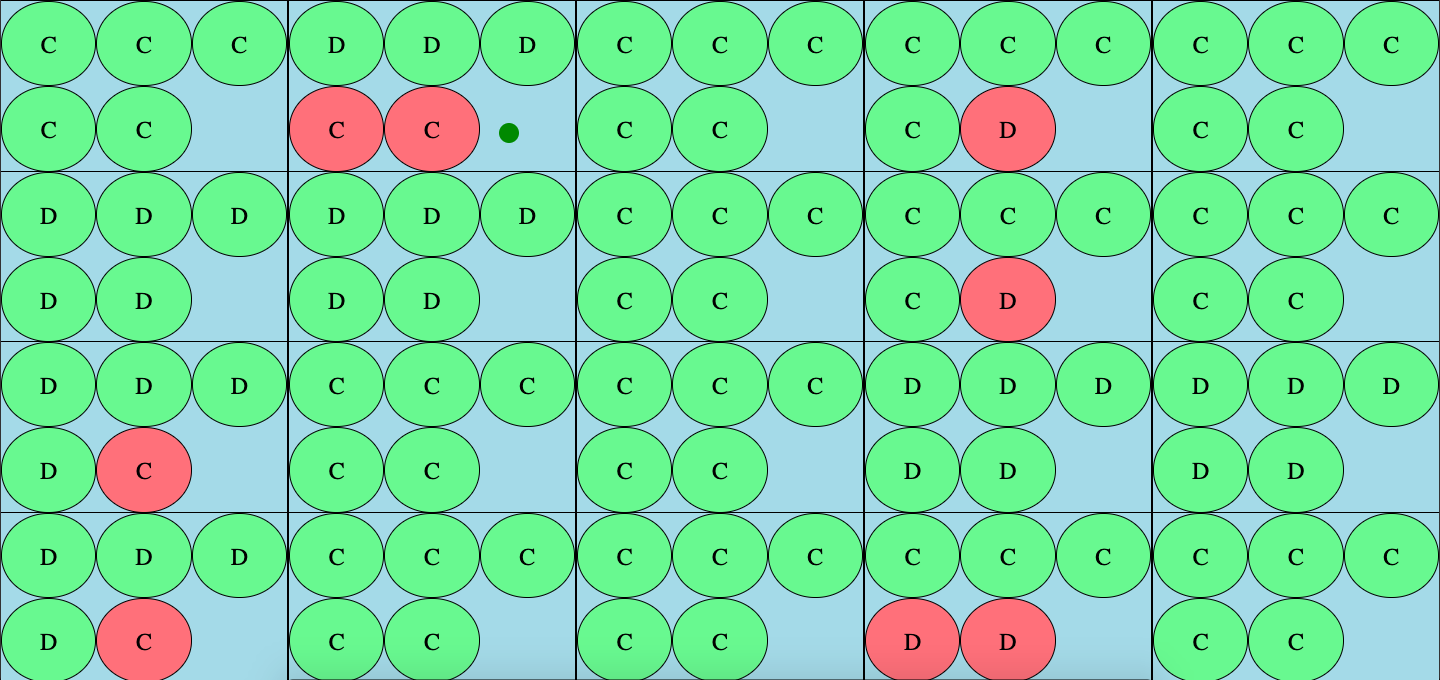
\includegraphics[width=0.8\columnwidth]{chapters/03_muifold/figures/user_study_lius.png}
  \caption{Modified Liu et al.'s test as shown to users.}
  \label{fig:user_study_lius}
\end{figure}


\subsection{Surveys}

For the experiment, participants were asked to fill out a pre- and
post-survey. The pre-survey asked for familiarity with smart
room environments and then asked for familiarity with the
following devices:

\begin{enumerate}
    \item Wiimote
    \item Kinect
    \item Bluetooth Pointer
    \item Mouse
    \item Trackpad
    \item Laser Pointer
    \item Cellphone with attached pointer hardware
    \item Cellphone with attached reflective panels (like VICON)
    \item Cellphone with no additional hardware
\end{enumerate}

The post-survey utilized the NASA Task Load 
Index~\cite{hart_development_1988} which asks users to rank
from ``Very Low'' to ``very High'' a range of topics which were:

\begin{enumerate}
    \item Mental Demand
    \item Physical Demand
    \item Temporal Demand
    \item Performance
    \item Effort
    \item Frustration
\end{enumerate}

In addition to the above, participants were given an open-ended
box to fill in any other comments they might have about the system.
During the experiment, researchers took a number of observational
comments about the participant.